\documentclass[letterpaper, 10 pt, journal, twoside]{IEEEtran}  % Use this command for final RAL version
%\documentclass[a4paper, 10pt, conference]{ieeeconf}      % Use this line for a4 paper

\IEEEoverridecommandlockouts                              % This command is only needed if
                                                          % you want to use the \thanks command

%\overrideIEEEmargins % Needed to meet printer requirements.

\usepackage{mathtools} 
\usepackage{graphicx,subcaption} % to use subfigure
\graphicspath{{img/}}
% To import svg, and automatic workflow with inkscape.
% But including svg also includes subfig which seems to collide with subfigure
% This gives the error main.tex|143 error| Undefined control sequence. \sf@counterlist
% Just remove deprecated subfigure, and use subcaptions instead...
%\usepackage[svgpath=img/]{svg}
% To import pgf figures.
\usepackage{pgf}
% To use svgscale before calling input on a pdf_tex file or svg
\usepackage{calc}
% To solve the issue of relative paths inside pgf.
\newcommand\inputpgf[2]{{
\let\pgfimageWithoutPath\pgfimage
\renewcommand{\pgfimage}[2][]{\pgfimageWithoutPath[##1]{#1/##2}}
\input{#1/#2}
}}

\usepackage{todonotes}
%\global\long\def\todoblue#1{\todo[inline,backgroundcolor=cyan]{#1}}
%\global\long\def\todogreen#1{\todo[inline,backgroundcolor=green]{#1}}
\usepackage{soul}

% To solve a bug with titlesec, and with makeidx
\usepackage{etoolbox}

\usepackage{amsmath} % To get math functionality
% Use amsmath to create my own definition equality symbol
\newcommand\defeq{\mathrel{\overset{\makebox[0pt]{\mbox{\tiny def}}}{=}}}
\usepackage{amssymb} % For nice math symbols
\usepackage{bm} % Better than \boldsymbol, use \bm
\usepackage[export]{adjustbox}% http://ctan.org/pkg/adjustbox
% To add tables with even width
\usepackage{tabularx}
\newcolumntype{Y}{>{\centering\arraybackslash}X} % To make columns content centered
\usepackage{tikz} % To draw
\usetikzlibrary{bayesnet} % To draw factor graphs in latex.

% Set variables for factor graph distances.
\newlength{\state} % Edge distance btw states
\setlength{\state}{1cm}

% For URLs
\usepackage{url}
% For mulicolumn
\usepackage{array}
% For copyright letters
\usepackage{textcomp}
% To avoid commands ignoring space after
\usepackage{xspace}
% To do nice minimalistic tables
% and better spacing above and below the various rules in the table
\usepackage{booktabs}
% To have footnotes in tables
\usepackage{tablefootnote}
% To allow for letters in enumerate (i, ii, ...)
\usepackage[shortlabels]{enumitem}

% For links
\usepackage{hyperref}
% Nice links and urls
\hypersetup{
    colorlinks,
    linkcolor={red!50!black},
    citecolor={blue!50!black},
    urlcolor={blue!80!black}
}

% Cleverer referencing
% Hyperref must be set before cleveref or cref won't work
\usepackage{cleveref}
%\crefformat{section}{\S#2#1#3} % Change section word for symbol
%\crefformat{subsection}{\S#2#1#3}
%\crefformat{subsubsection}{\S#2#1#3}

% Increase secnumdepth to also be able to reference paragraphs
\setcounter{secnumdepth}{6}

% For citations to be ordered
\usepackage[sort]{cite} % sorting is default actually

% useful comments
\usepackage{color}
\newcommand{\Rebuttal}[1]{\textcolor{black}{#1}}
\definecolor{orange}{RGB}{255,127,0}
\newcommand{\TR}[1]{\textcolor{orange}{{\\ \bf TR:}~#1}\\}
\newcommand{\LC}[1]{\textcolor{red}{{\bf LC:}~#1}}

% COLORS
\newcommand{\blue}[1]{{\color{blue}#1}}
\newcommand{\green}[1]{{\color{green}#1}}
\newcommand{\red}[1]{{\color{red}#1}}

% TO MANAGE REFERENCES
%============================================================================
\newcommand{\linkToPdf}[1]{\href{#1}{\blue{(pdf)}}}
\newcommand{\linkToPpt}[1]{\href{#1}{\blue{(ppt)}}}
\newcommand{\linkToCode}[1]{\href{#1}{\blue{(code)}}}
\newcommand{\linkToWeb}[1]{\href{#1}{\blue{(web)}}}
\newcommand{\linkToVideo}[1]{\href{#1}{\blue{(video)}}}
\newcommand{\award}[1]{\xspace} % {{\red{#1}}} % omit awards

\newcommand{\mysubsection}[1]{{\bf#1.}} % \subsection{}

%\title{
%Densifying Sparse VIO \\ A mesh-based approach using structural regularities
%}
\title{Semantic 3D Mesh VIO}

% Paper headers
\markboth{IEEE Intelligent Robots and Systems. Preprint Version.}
{Rosinol \MakeLowercase{\textit{et al.}}: Semantic 3D Mesh VIO}
% Use only for final RAL version

\author{Antoni Rosinol$^{1}$, Siyi Hu$^{1}$, Luca Carlone$^{1}$
\thanks{$^{1}$A.\,Rosinol, S.\,Hu and L.\,Carlone are with the Laboratory for
Information \& Decision Systems (LIDS), Massachusetts Institute of Technology, Cambridge, MA, USA,
{\sf \{arosinol,siyihu,lcarlone\}@mit.edu}}
\thanks{This work was partially funded by ARL DCIST CRA W911NF-17-2-0181.}}%

%\thanks{Manuscript received: September, 10, 2017; Revised December, 2, 2017; Accepted December, 4, 2017.} %Use only for final RAL version
%Use only for final RAL version.

\newcommand{\TODO}[1]{
\textcolor{orange}{{\textbf{TODO:}}~#1} % Comment this line to remove TODOs
}

%!TEX root = ../main.tex

% Shortcuts
\newcommand{\hide}[1]{}
\newcommand{\Figure}{Fig.~}%Use cref instead %Put the \ref next to \Figure: \Figure\ref{...}
\newcommand{\Section}{Sec.~}%Use cref instead %Put the \ref next to \Section \Section\ref{...}
\newcommand{\Equation}{Eq.~}%Use cref instead
\newcommand{\ie}{\emph{ie.~}}
\newcommand{\eg}{\emph{eg.~}}
\newcommand{\cf}{\emph{cf.~}}
\newcommand{\bdmath}{\begin{dmath}}%Use ultisnips instead for the following
\newcommand{\edmath}{\end{dmath}}
\newcommand{\beq}{\begin{equation}}
\newcommand{\eeq}{\end{equation}}
\newcommand{\bdm}{\begin{displaymath}}
\newcommand{\edm}{\end{displaymath}}
\newcommand{\bea}{\begin{eqnarray}}
\newcommand{\eea}{\end{eqnarray}}
\newcommand{\beal}{\beq \begin{array}{ll}}
\newcommand{\eeal}{\end{array} \eeq}
\newcommand{\beas}{\begin{eqnarray*}}
\newcommand{\eeas}{\end{eqnarray*}}
\newcommand{\ba}{\begin{array}} % Remember to add option, i.e. \ba{lcc}
\newcommand{\ea}{\end{array}}
\newcommand{\bpa}{\left(\ba} % Remember to add option, i.e. \bpa{lcc}
\newcommand{\epa}{\ea\right)}
\newcommand{\bit}{\begin{itemize}}
\newcommand{\eit}{\end{itemize}}
\newcommand{\ben}{\begin{enumerate}}
\newcommand{\een}{\end{enumerate}}
\newcommand{\bbmat}{\begin{bmatrix}}
\newcommand{\ebmat}{\end{bmatrix}}
\newcommand{\bpmat}{\begin{pmatrix}}
\newcommand{\epmat}{\end{pmatrix}}

% Operators
\DeclareMathOperator*{\argmin}{argmin}

% Groups, Domains, Sets
\newcommand{\SO}{\mathrm{SO}}
%\newcommand{\so}{\mathfrak{so}}
\newcommand{\SE}{\mathrm{SE}}
\newcommand{\se}{\mathfrak{se}}
\newcommand{\Sphere}{\mathrm{S}}
\newcommand{\su}{\mathfrak{su}}
\newcommand{\Real}{\mathbb{R}}
\newcommand{\Int}{\mathbb{Z}}
\newcommand{\ImageDomain}{\Omega}
\newcommand{\Surface}{\mathcal{S}}
\newcommand{\SEtwo}{\ensuremath{\mathrm{SE}(2)}\xspace}
\newcommand{\SEthree}{\ensuremath{\mathrm{SE}(3)}\xspace}
\newcommand{\Simthree}{\ensuremath{\mathrm{Sim}(3)}\xspace}
\newcommand{\SOtwo}{\ensuremath{\mathrm{SO}(2)}\xspace}
\newcommand{\SOthree}{\ensuremath{\SO(3)}\xspace}
\newcommand{\sothree}{\ensuremath{\so(3)}\xspace}
\newcommand{\Sthree}{\ensuremath{\Sphere^3}\xspace}
\newcommand{\Stwo}{\ensuremath{\Sphere^2}\xspace}
\newcommand{\sutwo}{\ensuremath{\su(2)}\xspace}
\newcommand{\setdef}[2]{ \{#1 \; {:} \; #2 \} }
\newcommand{\Pthree}{\ensuremath{\mathbb{P}^3}\xspace}
\newcommand{\Rthree}{\ensuremath{\mathbb{R}^3}\xspace}
\newcommand{\Rtwo}{\ensuremath{\mathbb{R}^2}\xspace}

% Calligraphic fonts
\newcommand{\calA}{{\cal A}}
\newcommand{\calB}{{\cal B}}
\newcommand{\calC}{{\cal C}}
\newcommand{\calD}{{\cal D}}
\newcommand{\calE}{{\cal E}}
\newcommand{\calF}{{\cal F}}
\newcommand{\calG}{{\cal G}}
\newcommand{\calH}{{\cal H}}
\newcommand{\calI}{{\cal I}}
\newcommand{\calJ}{{\cal J}}
\newcommand{\calK}{{\cal K}}
\newcommand{\calL}{{\cal L}}
\newcommand{\calM}{{\cal M}}
\newcommand{\calN}{{\cal N}}
\newcommand{\calO}{{\cal O}}
\newcommand{\calP}{{\cal P}}
\newcommand{\calQ}{{\cal Q}}
\newcommand{\calR}{{\cal R}}
\newcommand{\calS}{{\cal S}}
\newcommand{\calT}{{\cal T}}
\newcommand{\calU}{{\cal U}}
\newcommand{\calV}{{\cal V}}
\newcommand{\calW}{{\cal W}}
\newcommand{\calX}{{\cal X}}
\newcommand{\calZ}{{\cal Z}}

% Image
\newcommand{\Image}{\mathtt{I}}
\newcommand{\Depth}{\mathtt{D}}
\newcommand{\bearingvec}{\mathbf{f}}
\newcommand{\px}{\mathbf{u}} % Pixel
\newcommand{\pt}{\mathbf{p}} % 3D point
\newcommand{\depth}{d}
\newcommand{\proj}{\pi}

% Transformation
\newcommand{\T}{\mathtt{T}}
\newcommand{\R}{\mathbf{R}}
\renewcommand{\S}{\mathtt{S}}
\newcommand{\Identity}{\mathbf{I}}
\newcommand{\inv}{^{-1}}

% Matrices
\newcommand{\trace}[1]{\mathrm{tr}\left(#1\right)}

% Other
\newcommand{\residual}{\mathbf{r}}
\newcommand{\transpose}{\mathsf{T}} % consider using instead \rm T
\newcommand{\Zero}{\mathbf{0}}
\newcommand{\eye}{{\mathbf I}}
\renewcommand{\skew}{{\mathbf S}}
\newcommand{\Jac}{\mathtt{J}}
\newcommand{\Zthree}{\Zero_{3 \times 3}}
\newcommand{\Ithree}{\eye_{3 \times 3}}

% Imu
\newcommand{\rotvel}{\boldsymbol\omega}
\newcommand{\acc}{\mathbf{a}}
\newcommand{\rotvec}{\boldsymbol\phi}
\newcommand{\rotvecpert}{\delta\rotvec}
\newcommand{\rotvecang}{\varphi}	% rotation vector angle
\newcommand{\rotvecdir}{\mathbf{a}} % rotation vector direction
\newcommand{\tran}{\mathbf{p}}
\newcommand{\tranpert}{\delta\tran}
\newcommand{\vel}{\mathbf{v}}
\newcommand{\velpert}{\delta\vel}
\newcommand{\bias}{\mathbf{b}}
\newcommand{\biaspert}{\delta\bias}
\newcommand{\gravity}{\mathbf{g}}
\newcommand{\noise}{\boldsymbol\eta}
\newcommand{\VIO}{VIO\xspace}
\newcommand{\odometry}{navigation\xspace}
\newcommand{\tango}{{\rm Tango}\xspace}

% Quaternions
\newcommand{\Quat}{\ensuremath{\boldsymbol{q}}\xspace}

% Poses
\newcommand{\Pose}{\ensuremath{x}\xspace}
\newcommand{\PoseMeas}{\ensuremath{\tilde{x}}\xspace}
\newcommand{\PoseEst}{\ensuremath{\hat{x}}\xspace}

% Landmarks
\newcommand{\LandmarkSet}{\ensuremath{\calL}\xspace}

% Planes
\newcommand{\Plane}{\ensuremath{\boldsymbol{\pi}}\xspace}
\newcommand{\PlaneSet}{\ensuremath{\Pi}\xspace}
\newcommand{\PlaneMeas}{\ensuremath{\boldsymbol{\tilde\pi}}\xspace}
\newcommand{\PlaneEst}{\ensuremath{\boldsymbol{\hat\pi}}\xspace}

% Constraints
% Betweeen landmarks and planes
% Between planes
\newcommand{\parallelsum}{\mathbin{\!/\mkern-5mu/\!}} % for slanted parallellism // instead of ||

% Paper Specific
\newcommand{\Normal}{\ensuremath{\boldsymbol{n}}\xspace}
%\newcommand{\hl}[1]{ {\color{red} #1} }
\newcommand{\cut}[1]{\hl{cut? $\rightarrow$ #1}}
\newcommand{\Cov}{\mathbf{\Sigma}}
\newcommand{\at}[1]{^{(#1)}}
\newcommand{\expmap}{\mathrm{Exp}}
\newcommand{\logmap}{\mathrm{Log}}
\newcommand{\normsq}[2]{\left\|#1\right\|^2_{#2}}
\newcommand{\abs}[1]{\lvert#1\rvert}
\renewcommand{\d}{\text{d}}
\newcommand{\Rmean}{\R}
\newcommand{\Rrand}{\tilde\R}
\newcommand{\eq}{Eq.}
\newcommand{\eqs}{Eqs.}

\newcommand{\iSAMtwo}{iSAM2\xspace}
\newcommand{\MAP}{MAP\xspace}
\newcommand{\SVO}{SVO\xspace}
\newcommand{\GN}{GN\xspace}
\newcommand{\States}{\mathcal{X}}
\newcommand{\meascam}{\mathcal{C}}
\newcommand{\measimu}{\mathcal{I}}
\newcommand{\covprior}{\mathbf{\Sigma}}
\newcommand{\covimu}{\mathbf{\Sigma}}
\newcommand{\covcam}{\mathbf{\Sigma}_{\meascam}}
\newcommand{\World}{\text{W}}
\newcommand{\Imu}{\text{B}}
\newcommand{\Camera}{\text{C}}
\newcommand{\world}{\text{\tiny{W}}}
\newcommand{\imu}{\text{\tiny{B}}}
\newcommand{\camera}{\text{\tiny{C}}}
\newcommand{\cam}{{\scriptsize \text{c}}}
\newcommand{\accshort}{\tilde\acc(t)\!-\! \bias^a(t) \!-\! \noise^{ad}(t)}
\newcommand{\preintVar}{increments\xspace}
\newcommand{\biasFixedPreintVar}{bias-fixed increments\xspace}
\newcommand{\biasFixed}{\bar{\bias}}
\newcommand{\biasFixedDelta}{\Delta}
\newcommand{\biasHat}{\hat{\bias}}
\newcommand{\meters}{\rm{m}}
\newcommand{\preintRmeas}{\Delta\tilde\R}
\newcommand{\preintVmeas}{\Delta\tilde\vel}
\newcommand{\preintPmeas}{\Delta\tilde\tran}

% More paper specific
\newcommand{\F}{\mathcal{F}}

% smart factors
\newcommand{\pixel}{\mathbf{z}}
\newcommand{\pixelnoise}{\noise_{cam}}
\newcommand{\landmark}{\bm{\rho}}
\newcommand{\landmarkj}{\bm{\rho}_{l}}
\newcommand{\landpert}{\delta\landmark}
\newcommand{\posepert}{\delta\mathbf{T}}
\newcommand{\bvec}{\mathbf{b}}
\newcommand{\Amat}{\mathbf{A}}
\newcommand{\Bmat}{\mathbf{B}}
\newcommand{\Fmat}{\mathbf{F}}
\newcommand{\Emat}{\mathbf{E}}
\newcommand{\Qmat}{\mathbf{Q}}
%
\newcommand{\appendixRef}{Appendix\xspace}
\newcommand{\subimu}{{ij}}
\newcommand{\indmeas}{(i,j)}

% Jacobians
\newcommand{\DLog}{\mathtt{J}_{r}^{-1}}
\newcommand{\DExp}{\mathtt{J}_{r}}
\newcommand{\DExpk}{\mathtt{J}^k_{r}}
\newcommand{\jacobian}[2]{\frac{\partial #1}{\partial #2}}

% updates
\newcommand{\rup}{\rotvecpert}
\newcommand{\tup}{\tranpert}
\newcommand{\vup}{\velpert}
\newcommand{\bupa}{\tilde\delta{\bias^a_i}}
\newcommand{\bupg}{\tilde\delta{\bias^g_i}}

% Preintegrated measurements
\newcommand{\pRot}{\Delta\bar\R_{ij} } % integration value
\newcommand{\pRotk}{\Delta\bar\R_{ik} } % integration value
\newcommand{\pTran}{\Delta\bar\tran_{ij}}
\newcommand{\pVel}{\Delta\bar\vel_{ij}}
\newcommand{\pVelk}{\Delta\bar\vel_{ik}}
\newcommand{\mRot}{\Delta\tilde\R_{ij}} % measured
\newcommand{\mTran}{\Delta\tilde\tran_{ij}}
\newcommand{\mVel}{\Delta\tilde\vel_{ij}}
\newcommand{\Adjoint}{\mathtt{Ad}}

\newcommand{\biasCorrectedGyroMeas}{\tilde\rotvel(t) \!-\! \bias^g(t)}
\newcommand{\biasCorrectedAccMeas}{\tilde\acc(t) \!-\! \bias^a(t)}
\newcommand{\Rmeas}{\tilde\R}
\newcommand{\vmeas}{\tilde\vel}
\newcommand{\tmeas}{\tilde\tran}

% Factor graphs
\newcommand{\Factor}{\ensuremath{\phi}\xspace}

% Optimization
\newcommand{\TimeWindow}{\ensuremath{\Delta_t}\xspace}

% Euroc dataset
\newcommand{\Euroc}{EuRoC\xspace}


 % Shortcuts used by Forster15icra.

\begin{document}

\LC{add: ``Probabilistic Structure from Motion with Objects (PSfMO)''}
\LC{add: ``ObjectFusion: An Object Detection and Segmentation framework with RGB-D SLAM and Convolutional Neural Networks
G Tian, L Liu, JH Ri, Y Liu, Y Sun - Neurocomputing, 2019''}
\LC{add: [PDF] GEN-SLAM: Generative Modeling for Monocular Simultaneous Localization and Mapping
P Chakravarty, P Narayanan, T Roussel - arXiv preprint arXiv:1902.02086, 2019}

\LC{add: [PDF] GEOMetrics: Exploiting Geometric Structure for Graph-Encoded Objects
EJ Smith, S Fujimoto, A Romero, D Meger - arXiv preprint arXiv:1901.11461, 2019}

\LC{Mesh Based Semantic Modelling for Indoor and Outdoor Scenes
Julien P. C. Valentin1,3 Sunando Sengupta1,3 Jonathan Warrell1 Ali Shahrokni2 Philip H. S. Torr1}

\LC{work from Soatto}

\LC{https://journals.sagepub.com/doi/abs/10.1177/0278364919839761}

\maketitle
%\thispagestyle{empty}
%\pagestyle{empty}

%!TEX root = ../main.tex
\begin{abstract}
    We present a suite of algorithms and simulators with open-source implementations suitable for general Robotics development.
    As robotics is starting to have an increasingly important role with applications such as drone delivery and autonomous cars, it is ever more important to test, refine and provide a proof-of-concept of our algorithmic designs in a fast yet reliable way.
    With the advent of powerful desktop computers with multiple graphic cards and high-performance processors, we have the possibility to accurately simulate worlds that are always closer to being indistinguishable from the real world.
    Although we still have not reach the level where one might discard completely a real-life demonstration for the sake of proving the validity of a system, we are getting there at an exponential pace.
    Soon we might reach the point where we will have difficulties to decide what is real from what is computer-generated. If the reader is not convinced that this will happen, we suggest checking the latest developments in Generative Adversarial Networks \TODO{cite}.

    Classical implementations of Visual-Inertial Odometry (VIO) algorithms ignore semantic information of the scene, as they rely solely on sparse landmarks.
    Nevertheless, recent work has shown the advantage of using richer representations of the scene, such as 3D meshes, to extract higher-level information such as structural regularities.
    In this work, we show that a 3D mesh of the scene can be further utilized to accommodate semantic information, which enhances the mapping side of a classical VIO beyond a sparse and uninformative point-cloud.
    Towards this end, we use recent work on semidefinite programming and conditional random fields to generate semantic information in real-time on a single-core CPU.
\end{abstract}

% Keywords appear just beneath the abstract. Use only for final version.
\begin{IEEEkeywords}
Vision-Based Navigation, Semantic Segmentation.
\end{IEEEkeywords}

\vspace{-2em}
\section*{Supplementary Material}
Videos of the experiments: \TODO{Add video url}



%!TEX root = ../main.tex

\section{Introduction}
\label{sec:introduction}

% Drop letter for first word of the Introduction
% Use only for final version.
 \IEEEPARstart{T}{he} advent of drone racing competitions, both manned and unmanned, requires the estimation of the fastest possible trajectory through a given race track.
 Finding this optimal trajectory can be useful for human pilots, and their tacticians, to evaluate their performance and improve upon it.
 For example, the teams in the Red Bull Air Race \cite{redbull} make use of such information to train and perfect their maneuvers.
 In this same way, drones can autonomously follow a dynamically feasible trajectory with high accuracy.
 This is especially interesting for autonomous drone races such as the Alpha Pilot race \cite{AlphaPilot}.
 Therefore, being able to infer the optimal feasible trajectory could potentially make fully-autonomous drones beat human pilots.
 We are still not there, but great progress in this direction is being made \cite{delmerico2019we}.

{\bf Contributions.}
\begin{itemize}
  \item Formulation of the minimum-time problem for the specific problem of drone-racing through multiple gates.
  \item Presentation of a means to solve the problem using readily available software.
\end{itemize}

{\bf Paper Structure.}
%\Cref{sec:related_work} introduces related work with a similar objective as ours.
Section~\ref{sec:mathematical_formulation} presents the mathematical formulation of our approach, and discusses the assumptions made.
Section~\ref{sec:results} reports and discusses the experimental results.

%!TEX root = ../main.tex

\section{Related Work}
\label{sec:related_work}

\subsection{TODO}
\label{ssec:sota_vin}

\subsection{Optimal Control}
\label{ssec:sota_semantic_segmentation}
%!TEX root = ../main.tex

\section{Approach}
\label{sec:mathematical_formulation}

\TODO{Apprach}
We consider a stereo visual-inertial system and adopt a \emph{keyframe}-based approach~\cite{Leutenegger15ijrr}.
This section describes our VIO front-end and back-end.
Our front-end proceeds by building a 2D Delaunay triangulation over the 2D keypoints at each keyframe.
Then, the VIO back-end estimates the 3D position of each 2D keypoint, which we use to project the 2D triangulation into a 3D mesh.
While we incrementally build the 3D mesh, we restrict the mesh to the time-horizon of the VIO optimization, which we formulate in a fixed-lag smoothing framework~\cite{Qin17arxiv, Carlone17icra-vioAttention}.
The 3D mesh is further used to extract structural regularities in the scene that are then encoded as constraints in the optimization problem.

%%%%%%%%%%%%%%%%%%%%%%%%%%%%%%%%%%%%%%%%%%%%%%%%%%%%%%%%%%%%%%%%%%%%%%%%%%%%%%%%%%%%
\subsection{Front-end}
\label{ssec:frontend}

Our front-end has the same components as a keyframe-based indirect visual-inertial odometry pipeline\cite{Leutenegger15ijrr, Blosch15iros}, but it also incorporates a module to generate a 3D mesh, and a module to detect structural regularities from the 3D mesh.
We refer the reader to \cite[Sec. 4.2.1]{RosinolMT} for details on the standard modules used, and we focus here instead on the 3D mesh generation and regularity detection.

\subsubsection{3D Mesh Generation}
\label{sssec:3d_mesh_generation}

Building a consistent 3D Mesh of the environment using a sparse point cloud from VIO is difficult because (i) the 3D positions of the landmarks are noisy, and some are outliers; (ii) the density of the point cloud is highly irregular; (iii) the point cloud is constantly morphing: points are being removed (marginalized) and added, while the landmarks' positions are being updated at each optimization step.
Therefore, we avoid performing a 3D tetrahedralisation directly from the sparse 3D landmarks, which would require expensive algorithms, such as space carving \cite{Pan2009proforma}.

\subsubsection{3D Mesh Propagation}
While some algorithms update the mesh for a single frame \cite{Greene17iccv,Teixeira16iros}, we attempt to maintain a mesh over the receding horizon of the fixed-lag smoothing optimization problem (\cref{ssec:backend}), which contains multiple frames.
The motivation is three-fold: (i) A mesh spanning multiple frames covers a larger area of the scene, which provides more information than just the immediate field of view of the camera. (ii) We want to capture the structural regularities affecting any landmark in the optimization problem.
(iii) Anchoring the 3D mesh to the time-horizon of the optimization problem also bounds the memory usage, as well as the computational complexity of updating the mesh.

\paragraph{Temporal propagation} deals with the problem of updating the 3D mesh when new keypoints appear and/or old ones disappear in the new frame.

\paragraph{Spatial propagation} deals with the problem of updating the global 3D mesh when a new local 3D mesh is available, and when old landmarks are marginalized from the optimization's time-horizon.
We solve the first problem by merging the new local 3D mesh to the previous (global) mesh, by ensuring no duplicated 3D faces are present.

\subsubsection{Regularity Detection}
\label{sssec:regularity_detection}

\subsubsection{Data Association}
\label{sssec:data_association}

\subsection{Back-end}
\label{ssec:backend}

\subsubsection{State Space}
\label{sssec:state_space}

If we denote the set of all keyframes up to time $t$ by $\calK_t$, the state of the system $\mathbf{x}_i$ at keyframe $i\in\calK_t$, is described by the IMU orientation $\R_i$,
 position $\tran_i$, velocity $\vel_i$ and biases $\bias_i$:
\beq
\mathbf{x}_i \doteq [\R_i,\tran_i,\vel_i,\bias_i],
\eeq
where the pose $(\R_i, \tran_i) \in \SEthree$, $\vel_i \in \Real^3$, and $\bias_i = [\bias^g_i \;\; \bias^a_i] \in \Real^6$, and $\bias^g_i, \bias^a_i \in \Real^3$ are the gyroscope and accelerometer biases, respectively.

We will only estimate the 3D positions $\landmark_l$ for a subset $\Lambda_t$ of all landmarks $\LandmarkSet_t$ visible up to time $t$: $\{\landmark_l\}_{l\in\Lambda_t}$, where $\Lambda_t \subseteq \LandmarkSet_t$.
We will avoid optimizing over the rest of the landmarks $\LandmarkSet_t\setminus\Lambda_t$ by using a structureless approach, as defined in \cite[Sec. VII]{Forster17troOnmanifold}, which circumvents the need to add the landmarks' positions as variables in the state.
This allows to trade accuracy for speed; as the optimization’s complexity increases with the number of variables to be estimated.

The set $\Lambda_t$ corresponds to the landmarks which we consider to satisfy a structural regularity.
In particular, we are interested in co-planarity regularities, which we introduce in \cref{sssec:regularity_constraints}.
Since we need the explicit landmark variables to formulate constraints on them, we avoid using a structureless approach for these landmarks.

Finally, the co-planarity constraints between the landmarks $\Lambda_t$ require the modelling of the planes $\PlaneSet_t$ in the scene.
Therefore, the variables to be estimated comprise the state of the system $\{\mathbf{x}_i\}_{i\in\calK_t}$, the landmarks which we consider to satisfy structural regularities $\{\landmark_l\}_{l\in\Lambda_t}$, and the planes $\{\Plane_\pi\}_{\pi\in\PlaneSet_t}$.
The variables to be estimated at time $t$ are:

\begin{equation}
  \calX_t \doteq \displaystyle\left\{\mathbf{x}_i, \landmark_l, \Plane_\pi\right\}_{i\in\calK_t, l\in\Lambda_t, \pi\in\Pi_t}
  \label{eq:state_vector}
\end{equation}

Since we are taking a fixed-lag smoothing approach for the optimization, we limit the estimation problem to the sets of variables that depend on the keyframes in a time-horizon of size $\TimeWindow$.
To avoid cluttering the notation, we skip the dependence of the sets $\calK_t$, $\Lambda_t$ and $\Pi_t$ on the parameter $\TimeWindow$.

By reducing the number of state variables to a given window of time $\TimeWindow$, we will make the optimization problem tractable and solvable in real-time.

\subsubsection{Measurements}
\label{sssec:measurements}

The input for our system consists on measurements from the camera and the IMU.
We define the image measurements at keyframe $i$ as $\meascam_i$ .
The camera can observe multiple landmarks $l$, hence $\meascam_i$ contains multiple image measurements $\mathbf{z}_{i}^{l}$,
 where we distinguish the landmarks that we will use for further structural regularities $\mathbf{z}_{i}^{l_{c}}$ (where the index $c$ in $l_c$ stands for constrained landmark),
  and the landmarks that will remain as structureless $\mathbf{z}_{i}^{l_s}$ (where the $s$ in the index of $l_s$ stands for structureless).
We represent the set of IMU measurements acquired between two consecutive keyframes $i$ and $j$ as  $\measimu_\subimu$.
Therefore, we define the set of measurements collected up to time $t$ by $\mathcal{Z}_t$:
\begin{equation}
  \mathcal{Z}_t \doteq \{\meascam_i, \measimu_\subimu\}_{\indmeas \in \mathcal{K}_t}.
  \label{eq:measurements}
\end{equation}


\subsubsection{Factor Graph Formulation}
\label{sssec:factor_graph}

We want to estimate the posterior probability $p(\calX_t|\mathcal{Z}_t)$ of our state $\calX_t$, as defined in \cref{eq:state_vector}, using the set of measurements $\mathcal{Z}_t$, defined in \cref{eq:measurements}.
Using standard independence assumptions between measurements and states, we arrive to the formulation in \cref{eq:factor_form}, where we grouped the different terms in factors $\phi$:
\begin{subequations}\label{eq:factor_form}
  \begin{align}
    &p(\calX_t|\mathcal{Z}_t) \overset{(a)}{\propto} p(\mathcal{Z}_t|\calX_t)p(\calX_t) \nonumber\\
    &= \phi_0(\mathbf{x}_0)\prod_{l_c\in\Lambda_t}\prod_{\pi\in\Pi_t}\!\phi_{\mathcal{R}}(\bm{\rho}_{l_c}, \bm\pi_\pi)^{\delta(l_c, \pi)} \label{eq:factor_form_a}\\
    &\quad\quad\quad\quad\prod_{(i,j)\in\calK_t}\!\!\!\phi_{\text{IMU}}(\mathbf{x}_i, \mathbf{x}_j) \label{eq:factor_form_b}\\
    &\prod_{i\in\calK_t}\prod_{l_c\in\meascam_i^c}\!\phi_{l_c}(\mathbf{x}_i, \bm{\rho}_{l_c}) \!\!\prod_{i\in\calK_t}\prod_{l_s\in\meascam_i^s}\!\phi_{l_s}(\mathbf{x}_i) \label{eq:factor_form_c}
  \end{align}
\end{subequations}
where we apply the Bayes rule in (a), and ignore the normalization factor over the measurements since it will not influence the result (\cref{sssec:map_estimation}).

\Cref{eq:factor_form_a} corresponds to the prior information we have over the state $p(\calX_t)$.
In this term, we encode regularity constraints between landmarks $\bm\rho_{l_c}$ and planes $\pi$, which we denote by $\phi_{\mathcal{R}}$.
We also introduce the data association term $\delta(l_c, \pi)$, which returns a value of 1 if the landmark $l_c$ is associated to the plane $\pi$, 0 otherwise.
We explain in \cref{sssec:data_association} how the data association is done.
The factor $\phi_0$ represents a prior on the first pose of the optimization's time-horizon.

In \cref{eq:factor_form_b}, we have the factor corresponding to the IMU measurements, which depends only on the consecutive keyframes $(i, j)\in\calK_t$.

Finally, \cref{eq:factor_form_c} encodes the factors corresponding to the camera measurements.
Since we want to distinguish between landmarks that are involved in structural regularities ($l_c$) and landmarks that are not ($l_s$), we split the product over $C_i$;
where we write $l_s\in \meascam_i^s$ or $l_c\in \meascam_i^c$ when a landmark $l_s$ or $l_c$, respectively, is seen at keyframe $i$ by the camera. Note that $\meascam_i = \meascam_i^c \cup \meascam_i^s$ and $\meascam_i^c \cap \meascam_i^s = \emptyset$.

In \cref{fig:factor_graph_s_p_r_1}, we use the expresiveness of factor graphs \cite{Kschischang01it} to show the actual dependencies between the variables in \cref{eq:factor_form}\footnote{We will use the notation proposed in \cite{Dietz10directed} to represent the factor graph.}.

\begin{figure}[h]
  \centering
  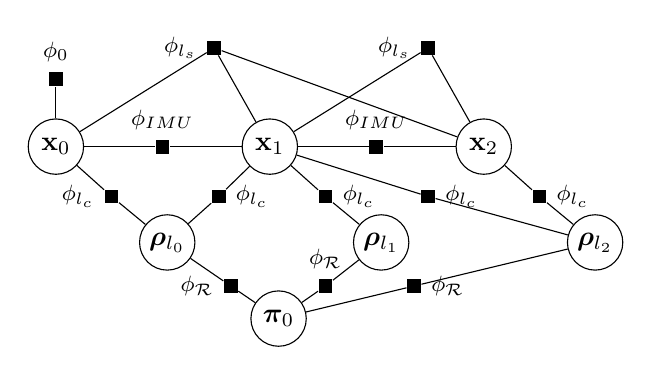
\begin{tikzpicture}
    % X nodes
    \node[latent] (x0) {$\mathbf{x}_0$};
    \node[latent, right= of x0, xshift=\state] (x1) {$\mathbf{x}_1$};
    \node[latent, right= of x1, xshift=\state] (x2) {$\mathbf{x}_2$};

    % L nodes
    \node[latent, below=0.5 of x0, xshift=1.414\state] (l0) {$\bm\rho_{l_0}$};
    \node[latent, below=0.5 of x1, xshift=1.414\state] (l1) {$\bm\rho_{l_1}$};
    \node[latent, below=0.5 of x2, xshift=1.414\state] (l2) {$\bm\rho_{l_2}$};

    % Pi nodes
    \node[latent, below=0.25 of l0, xshift=1.414\state] (pi0) {$\bm\pi_0$};

    % Prior on X0
    \factor[above=of x0, xshift=0\state] {x0prior} {above:$\phi_{0}$} {x0} {}; %

    % Pre-integrated IMU
    % For X0 - X1
    \factor[right=of x0, xshift=0.5\state] {x0-x1} {above:$\phi_{IMU}$} {x0, x1} {}; %
    % For X1 - X2
    \factor[right=of x1, xshift=0.5\state] {x1-x2} {above:$\phi_{IMU}$} {x1, x2} {}; %

    % Landmark observations
    % For L0
    \factor[below=0.18 of x0, xshift=0.707\state] {x0-l0} {left:$\phi_{l_c}$} {x0, l0} {}; %
    \factor[below=0.18 of x1, xshift=-0.650\state] {x1-l0} {right:$\phi_{l_c}$} {x1, l0} {}; %

    % For L1
    \factor[below=0.18 of x1, xshift=0.707\state] {x1-l1} {right:$\phi_{l_c}$} {x1, l1} {}; %

    % For L2
    \factor[below=0.18 of x2, xshift=0.707\state] {x2-l2} {right:$\phi_{l_c}$} {x2, l2} {}; %
    \factor[below=0.18 of x2, xshift=-0.707\state] {x1-l2} {right:$\phi_{l_c}$} {x1, l2} {}; %

    % For structureless
    \factor[above=0.8of x1, xshift=-0.707\state] {x0-x1-x2} {left:$\phi_{l_s}$} {x0, x1,x2} {}; %
    \factor[above=0.8of x2, xshift=-0.707\state] {x1-x2} {left:$\phi_{l_s}$} {x1,x2} {}; %

    % For plane
    % plane-landmarks
    \factor[below=0.1 of l0, xshift=0.807\state] {pi0-l0-l1} {left:$\phi_{\mathcal{R}}$} {l0, pi0} {}; %
    \factor[below=0.1of l1, xshift=-0.707\state] {pi0-l1} {above:$\phi_{\mathcal{R}}$} {l1, pi0} {}; %
    \factor[below=0.1of l2, xshift=-2.3\state] {pi0-l2} {right:$\phi_{\mathcal{R}}$} {l2, pi0} {}; %
  \end{tikzpicture}
  \caption{VIO factor graph combining Structureless ($\phi_{l_s}$), Projection ($\phi_{l_c}$) and Regularity ($\phi_{\mathcal{R}}$) factors (SPR).
The factor $\phi_{\mathcal{R}}$ encodes relative constraints between a landmark $l_i$ and a plane $\pi_0$.}
  \label{fig:factor_graph_s_p_r_1}
\end{figure}

\subsubsection{MAP Estimation}
\label{sssec:map_estimation}
Since we are only interested in the most likely state $\calX_t$ given the measurements $\mathcal{Z}_t$, we calculate the \emph{maximum a posteriori} (MAP) estimator $\calX_t^{\text{MAP}}$.
Maximizing $\calX_t^{\text{MAP}}$ is nevertheless not as convenient as minimizing the negative logarithm of the posterior probability, which, using \cref{eq:factor_form}, simplifies to \cref{eq:simplified_map} for zero-mean Gaussian noise:

\begin{equation}
  \begin{split}
   &\calX_t^{\text{MAP}} = \arg\min_{\calX_t} \normsq{\mathbf{r}_0}{\Sigma_0} + \!\!\!\sum_{l_c\in\Lambda_t}\!\sum_{\pi\in\Pi_t}\delta(l_c, \pi)\normsq{\mathbf{r}_{\mathcal{R}}}{\Sigma_{\mathcal{R}}} \\
                  &+ \!\!\!\!\!\sum_{(i,j)\in\calK_t}\!\!\!\normsq{\mathbf{r}_{\measimu_\subimu}}{\Sigma_{ij}} \!\!\! + \!\!\! \sum_{i\in\calK_t}\!\!\Bigg\{\!\sum_{l_c\in\meascam_i} \normsq{\mathbf{r}_{\mathcal{C}_{i}^{l_c}}}{\Sigma_\mathcal{C}} \!\!\! + \!\!\! \sum_{l_s\in\meascam_i} \normsq{\mathbf{r}_{\mathcal{C}_{i}^{l_s}}}{\Sigma_\mathcal{C}}\!\!\Bigg\} \\
  \end{split}
  \label{eq:simplified_map}
\end{equation}
where $\mathbf{r}$ represents the residual errors, and $\mathbf{\Sigma}$ the covariance matrices.
We refer the reader to \cite[Sec. VI, VII]{Forster17troOnmanifold} for the actual formulation of the preintegrated IMU factors $\phi_{\text{IMU}}$ and structureless factors $\phi_{l_s}$, as well as the underlying residual functions $\mathbf{r}_{\text{IMU}}$, $\mathbf{r}_{C_i^{l_s}}$.
For the projection factors $\phi_{l_c}$, we use a standard monocular and stereo reprojection error formulation as in \cite{Carlone17icra-vioAttention}.

\subsubsection{Regularity Constraints}
\label{sssec:regularity_constraints}

For the regularity factors $\phi_{\mathcal{R}}$, we use a co-planarity constraint between a landmark $\bm\rho_{l_c}\in\mathbb{R}^3$ and a plane $\pi = \{\bm{n}, d\}$, where $\bm{n}$ is the normal of the plane, which lives in the $\Stwo\doteq\{\mathbf{n} = (n_x, n_y, n_z)^T \big| \|\mathbf{n}\| = 1\}$ manifold, and $d\in\mathbb{R}$ the distance to the origin:
$\textstyle\residual_{\mathcal{R}} = \bm{n} \cdot \bm{\rho}_{l_c} - d$.
Representing a plane by its normal and distance to the origin is an over-parametrization that will lead to an information matrix that is singular.
This is not amenable for Gauss-Newton optimization, since it leads to singularities in the normal equations~\cite{Kaess15icra}.
%which requires the inverse of the information matrix.
To avoid the over-parametrization problem, we optimize in the tangent space $T_{\Normal}S^2 \sim \Real^{2}$ % \doteq \big\{\hat\xi \in \Real^3 | \Normal^T \hat\xi = 0\big\}$
of $S^2$ and define a suitable retraction $\calR_{\Normal}(\bm{v}): T_{\Normal}S^2 \in \mathbb{R}^2 \rightarrow \Stwo$
to map changes in the tangent space to changes to the normals in $\Stwo$~\cite{Forster17troOnmanifold}. % to obtain a minimal parametrization for the
In other words, we rewrite the residuals as:
\begin{equation}
  % \residual_\mathcal{R}(\Normal, d) = \Normal^\transpose \cdot \landmark - d \Leftrightarrow
  \residual_\mathcal{R}(\bm{v},d) = \calR_{\Normal}(\bm{v})^\transpose \cdot \landmark - d
  \label{eq:coplanarity_constraint}
\end{equation}
and optimize with respect to the minimal parametrization $\bm{v}$.
 This is similar to the proposal of Kaess~\cite{Kaess15icra}, but we work on the manifold $\Stwo$, while Kaess adopts a quaternion parametrization.
Note that, a single co-planarity constraint, as defined in \cref{eq:coplanarity_constraint}, is not sufficient to constrain a plane variable, and a minimum of three are needed instead.
Nevertheless, degenerate configurations exist, e.g.~three landmarks on a line would not fully constrain a plane.
Therefore, we ensure that a plane candidate has a minimum number of constraints before adding it to the optimization problem.
%\subsubsection{Robust Cost Functions}
%\label{sssec:robust_cost_functions}
\TODO{Do we need to mention robust cost functions at all? I think so, reviews were picky about outliers!}
%Running a feature-based VIO pipeline over planar surfaces, such as walls, has the inconvenience that few features are usually present (i.e. textureless walls), or features are easy to wrongly associate against each other (i.e. a wall with high-frequency texture).
%This can lead to certain estimated landmarks being plainly wrong (outliers), and can consequently corrupt the estimated variables in the optimization problem.
%This is especially problematic in least-squares optimization, which is particularly sensitive to outliers.

%For this reason, we will be using a robust cost function for both the projection and regularity residuals.
%In particular, we found the Huber norm to yield the best results, while we also experimented with the Tukey norm.
%More details on the norm's formulations can be found in \cite{Zhang97ivc}.
%\TODO{Someone may ask why we did not use a robust cost function for structureless factors? And I do not fully understand the underlying mechanism to avoid outliers as it is in our pipeline right now for smart factors...}

%%%%%%%%%%%%%%%%%%%%%%%%%%%%%%%%%%%%%%%%%%%%%%%%%%%%%%%%%%%%%%%%%%%%%%%%%%%%%%%%%%%%

%!TEX root = ../main.tex

\section{Experimental Results}
\label{sec:results}

%!TEX root = ../main.tex

\section{Conclusion}
\label{sec:conclusions}

We have first presented a nonlinear model of a quadcopter suitable for an accurate representation of the dynamics involved in drone racing.
Then, we have formulated a minimum time optimal control problem in order to estimate the sequence of states and control inputs to finish the race in a minimum amount of time.
Finally, this paper considers the addition of conic constraints on the velocity of the drone to explicitly encode the fact that the drone must fully traverse a gate before heading to the next one.
The results achieved are promising and can be potentially used as a benchmark to assess how close to optimality other approaches are.

%\addtolength{\textheight}{-11cm}   % This command serves to balance the column lengths
                                  % on the last page of the document manually. It shortens
                                  % the textheight of the last page by a suitable amount.
                                  % This command does not take effect until the next page
                                  % so it should come on the page before the last. Make
                                  % sure that you do not shorten the textheight too much.


%\section*{Acknowledgments}

\bibliographystyle{IEEEtran} % use IEEEtran.bst style
\bibliography{bibliography}

%\addtolength{\textheight}{0cm}   % This command serves to balance the column lengths
%\newpage
%\input{./chapters/appendix_content.tex}

\end{document}
